\section{Einleitung}
Dies soll eine \LaTeX{} -Vorlage für den persönlichen Gebrauch werden. Sie hat weder einen Anspruch auf Richtigkeit,
noch auf Vollständigkeit. Die Quellen liegen auf Github zur allgemeinen Verwendung. Verbesserungen sind jederzeit willkommen.

\subsection{Zielsetzung}
Kleiner Reminder für mich in Bezug auf die Dinge, die wir bei der Thesis beachten sollten und \LaTeX{}-Vorlage für die Thesis.

\subsection{Aufbau der Arbeit}
Kapitel 2 enthält die Inhalte des Thesis-Days und alles, was zum inhaltlichen erstellen der Thesis relevant sein könnte.
Kapitel 3 wichtige Anmerkungen zu \LaTeX{}, wobei die wirklich wichtigen Dinge im Quelltext dieses Dokumentes stehen.

\begin{figure}[htbp]
    \begin{center}
        \raggedright\caption{Verzeichnisstruktur der \LaTeX-Datein}
        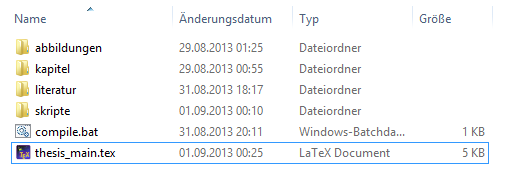
\includegraphics[width=1\textwidth]{verzeichnisStruktur}
        \captionsetup{width=1.0\textwidth}
        \capquelle{https://github.com/andygrunwald/FOM-LaTeX-Template}\label{figur-k1}
    \end{center}
\end{figure}
